\chapter{Mixed-Bag Solver Overview}\label{chap:mixedBagSolver}

When humans solves jigsaw puzzles, it is common for them to try to correctly assemble small regions of the puzzle and then merge those smaller regions to form larger regions.  The Mixed-Bag Solver presented in this thesis is based of this solving strategy.  The solver consists of five distinct stages, namely: segmentation, stitching, hierarchical clustering of segments, seed piece selection, and final assembly.  The flow of the algorithm is shown in Figure~\ref{fig:multipuzzleSolverArchitecture}; the pseudocode for the solver, including the input(s) and output of each stage is shown in Algorithm~\ref{alg:mixedBagSolver}.  The techniques used by the Mixed-Bag Solver are valid for Type~1, Type~2, and Mixed-Bag puzzles.  

The following subsections describe each of Mixed-Bag Solver's stages/subfunctions.  It also discusses the assembler (not shown in Figure~\ref{fig:multipuzzleSolverArchitecture}), which is a separate but associated component of the architecture.

\begin{figure}[ht!]
	\centering
		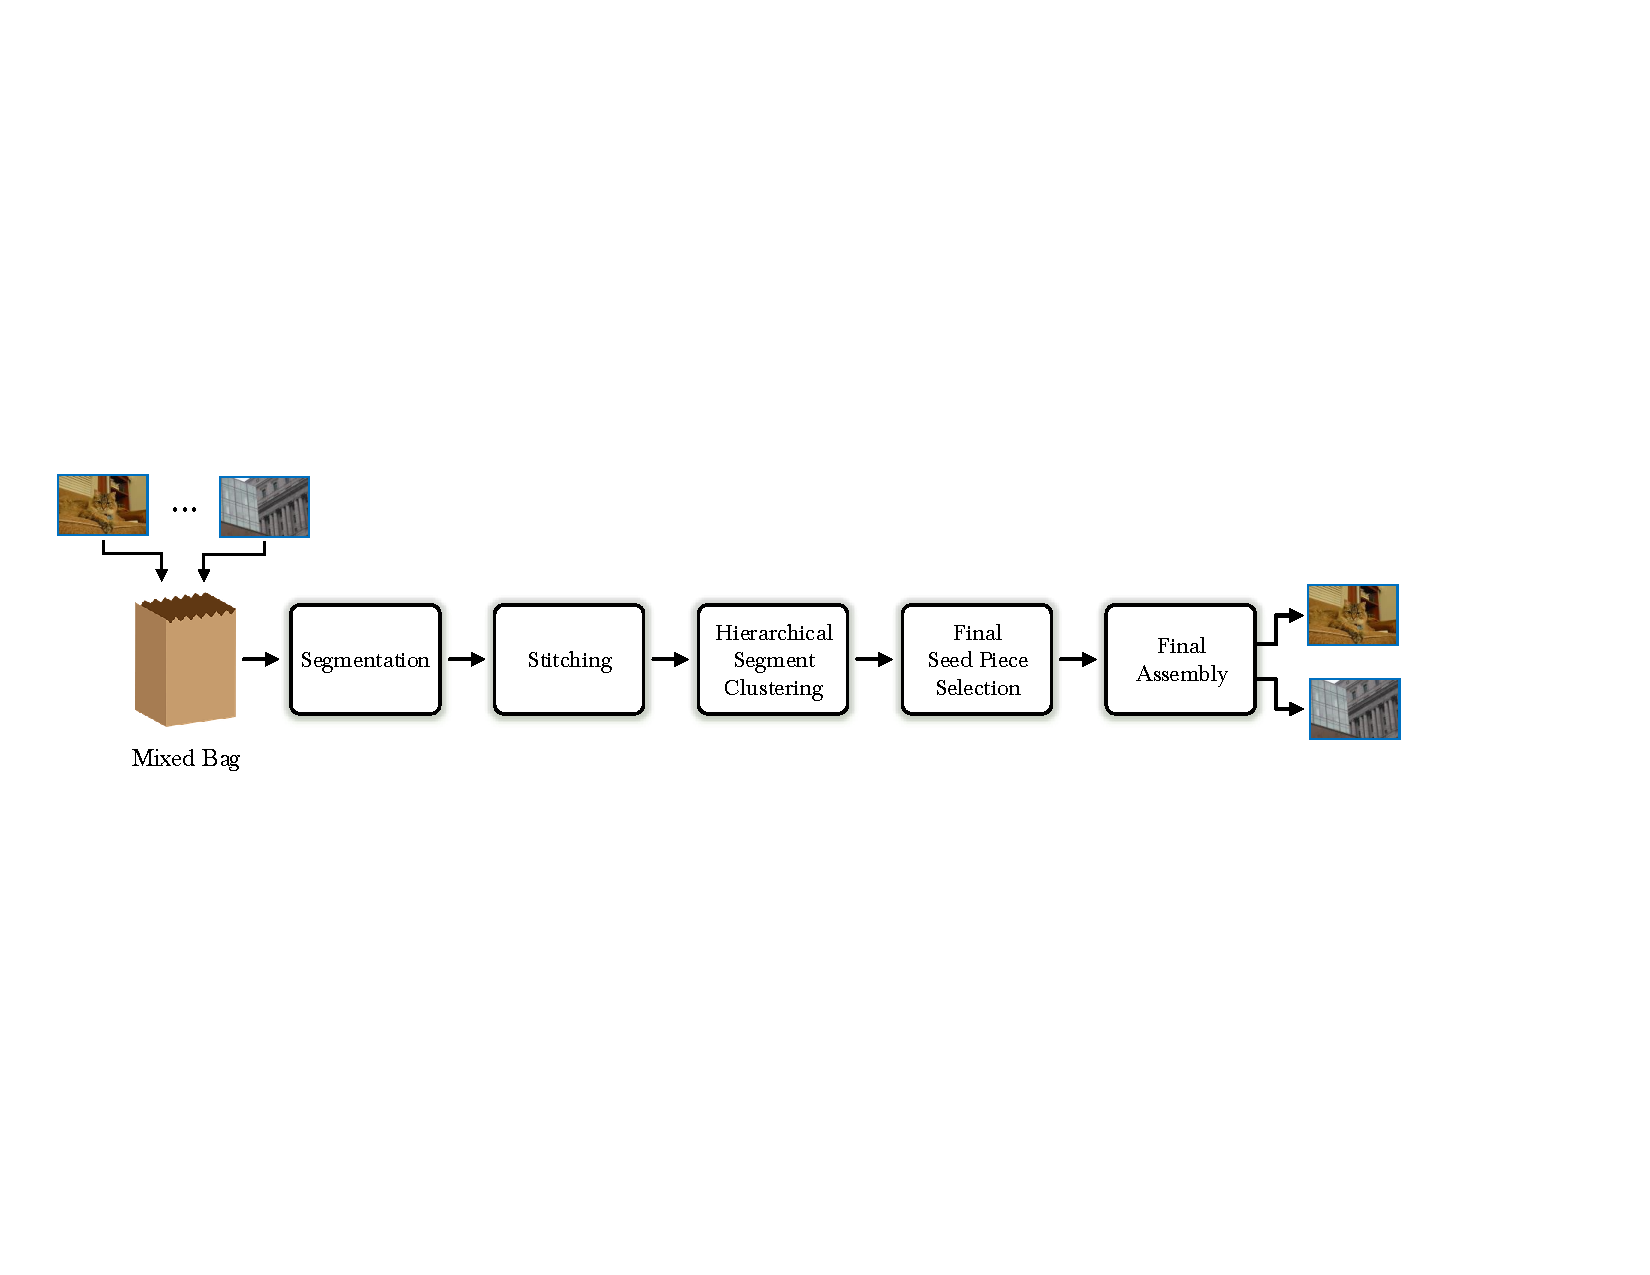
\includegraphics[width=1.0\textwidth]{images/cropped_algorithm_structure_overview.pdf}
	\caption{Components of the Mixed-Bag Puzzle Solver}\label{fig:multipuzzleSolverArchitecture}
\end{figure}

\begin{algorithm}[tb]
\caption{Pseudocode for the Mixed Bag Solver}\label{alg:mixedBagSolver}
\begin{algorithmic}[1]
\Function{MixedBagSolver}{$all\_pieces$}
    \State $solved\_segments \gets \textproc{Segmentation}\text{(} all\_pieces \text{)}$
	\State $overlap\_matrix \gets \textproc{Stitching}\text{(} solved\_segments \text{, } all\_pieces \text{)}$
	\State $clusters \gets \textproc{HierarchicalClustering} \text{(}solved\_segments \text{, } overlap\_matrix \text{)}$
	\State $puzzle\_start\_pieces \gets \textproc{FindStartingPieces} \text{(} clusters \text{)}$
	\State $solved\_puzzles \gets \textproc{RunFinalAssembly} \text{(} puzzle\_start\_pieces \text{, } all\_pieces \text{)}$
    \State \Return $solved\_puzzles$
\EndFunction
\end{algorithmic}
\end{algorithm}

\section{Assembler}\label{sec:SolverAssembler}

The assembler assigns the placement (and optionally rotation) of the puzzle pieces in the solved puzzle.  The Mixed-Bag Solver's architecture is largely independent of the particular assembler used.  Hence, any improvements or modifications to the assembler can be directly incorporated into the Mixed-Bag Solver to improve the solver's performance.  What is more, if a particular assembler performs better than others for a particular application, the assemblers can be interchanged.  This provides the Mixed-Bag Solver with significant flexibility and upgradability to maximize performance across a wide range of applications.

For all experiments in this thesis, the assembler proposed proposed by Paikin~\& Tal~\cite{paikin2015}.  As mentioned in Chapter~\ref{chap:previousWork}, their assembler is the current state of the art and is one of the few algorithms that natively supports Mixed-Bag puzzles.

\subsection{Assembler Time Complexity}\label{sec:assemblerTimeComplexity}

Paikin~\& Tal's assembler relies on a set of inter-puzzle piece distance and similarity metrics.  Similar to all other jig swap solvers, these distances are calculated between all pairs of possible pieces, making the time complexity of this stage at $O(n^2)$, where $n$ is the number of puzzle pieces.  If an input image has sufficient inter-piece variation, then assembly is expected to take $Theta(n \text{lg}(n)$ as a heap is used to determine the next piece to be placed.  However, if most pieces are sufficient similar that there are fewer best buddies (see Chapter~\ref{chap:previousWork}, then assembly can be as slow as $O(n^3)$ as the inter-piece similarity may need to be recalculated after each piece is placed.

Assembly only occurs once in Paikin~\& Tal's algorithm.  In the Mixed-Bag Solver, assembly is run at least once during segmentation stage (usually more) and is run again during the final assembly stage.  Hence, while the Mixed-Bag Solver will necessarily take longer to execute than Paikin~\& Tal's algorithm, the Mixed-Bag Solver's time complexity is the same.

\subsection{Assembler Implementation}\label{sec:assemblerImplementation}

Paikin~\& Tal wrote their algorithm in Java, and as of this prublication, their source code has not been released.  Hence, their algorithm was implemented as part of this thesis based off of the description in~\cite{paikin2015}.  This thesis' implementation is in the Python programming language and is fully open-source.  No execution time comparisons between their algorithm and the Mixed-Bag Solver are included with this thesis since Java is generally significantly faster than Python \cite{pythonJavaComparison}.

\section{Segmentation}\label{sec:Segmentation}

As detailed in Algorithm~\ref{alg:mixedBagSolver}, segmentation stages takes as input only the bag of puzzle pieces created from the original images; unlike all other solvers to date, this algorithm takes no other inputs.  The role of segmentation is to a basic provide structure to the unordered input.  This is done by partitioning the pieces into disjoint sets, referred to here as segments.  These segments are groups of puzzle pieces where there is a high degree of confidence that the pieces are assembled correctly.

Algorithm~\ref{alg:segmentation} outlines the basic segmentation framework; the implementation is iterative and will have one or more rounds.  In each round, all pieces not yet assigned to a saved segment are assembled as if they all belong to a single ground-truth image.  This strategy eliminates the need to make any assumptions regarding the input at this early stage.  What is more, it is expected that pieces from the same input puzzle may be assigned to multiple disjoint segments.  Section~\ref{sec:hierarchicalClustering} describes how these segments are merged using hierarchical clustering.

After the puzzle is assembled in a given round, the solved puzzle is then partitioned into segments; the segmentation procedure is described in Section~\ref{sec:segmentPuzzle}.  Assuming the largest segment exceeds the minimum allowed size\footnote{For this thesis, it was observed that a minimum segment size of 7 provided the best balance between solution quality and algorithm execution time.}, it is passed to the Stitching stage described in Section~\ref{sec:stitching}.  Similarly, the term ``\textit{$\alpha$}'' in Algorithm~\ref{alg:segmentation} dictates the segments in a given segmentation round, other than the largest one, that are also passed to the next stage of the Mixed-Bag Solver.  In this thesis, \textit{$\alpha$} was set to 0.5, meaning any segment that was at least half the size of the largest segment in that round is saved.  This scalar value provides sufficient balance between finding the largest possible segments for analysis and limiting overall execution time.

Once a piece is assigned to a saved segment, it is removed from the set of unassigned pieces.  Hence, those pieces will not be placed in the next segmentation round.  Segmentation continues until all pieces have been assigned to sufficiently large segments, or no segment exceeds the minimum allowed segment size.

\begin{algorithm}[tb]
\caption{Pseudocode for the Segmentation Algorithm}\label{alg:segmentation}
\begin{algorithmic}[1]
\Function{Segmentation}{$all\_pieces$}
    \State $saved\_segments \gets \{ \}$
    \State $unassigned\_pieces \gets \{ all\_pieces \}$
    \Loop
        \State $solved\_puzzle \gets \textproc{RunSinglePuzzleAssembly}(unassigned\_pieces)$
        \State $puzzle\_segments \gets \textproc{SegmentPuzzle}(solved\_puzzle)$
\item[]
        \State $max\_segment\_size \gets \text{maximum size of segment in } solved\_segments$
        \If{$max\_segment\_size \text{ < } smallest\_allowed$}
			\State \Return $saved\_segments$
        \EndIf
\item[]
        \ForEach{$segment \in puzzle\_segments$}
            \If{$|segment| \text{ > } \alpha \times max\_segment\_size$}
                \State $\text{add } segment \text{ to } saved\_segments$
                \State $\text{remove pieces in } segment \text{ from } unassigned\_pieces$
            \EndIf
        \EndFor
	\EndLoop
\EndFunction
\end{algorithmic}
\end{algorithm}

\subsection{The \textproc{SegmentPuzzle} Function}\label{sec:segmentPuzzle}

The \textproc{SegmentPuzzle} function shown in Algorithm~\ref{alg:segmentPuzzle} is adapted from the kernel growing segmentation procedure proposed by Pomeranz \textit{et al.}, where it was shown to have greater than 99.7\% accuracy identifying genuine neighbors \cite{pomeranz2011}. The kernel of each segment is a single seed piece.

\begin{algorithm}[tb]
\caption{Pseudocode to Segment a Solved Puzzle}\label{alg:segmentPuzzle}
\begin{algorithmic}[1]
\Function{SegmentPuzzle}{$solved\_puzzle$}
    \State $puzzle\_segments \gets \{ \}$
    \State $unassigned\_pieces \gets \{ \text{all pieces in } solved\_puzzle \}$
\item[]
    \While{$|unassigned\_pieces| \text{ > } 0$}
        \State $segment \gets \text{ new empty segment}$
        \State $seed\_piece \gets \text{next piece in } unassigned\_pieces$
        \State $queue \gets [seed\_piece]$
\item[]
        \While{$|queue| \text{ > } 0$}
            \State $piece \gets \text{next piece in } queue$
            \State $\text{add } piece \text{ to } segment$
\item[]
            \ForEach{$neighbor\_piece \text{ of } piece$}
            	\If{$\textproc{IsBestBuddies}(neighbor\_piece, piece)$}
            		\State $\text{add } neighbor\_piece \text{ to } \textit{queue}$
            		\State $\text{remove } neighbor\_piece \text{ from } unassigned\_pieces$
            	\EndIf
            \EndFor
        \EndWhile
\item[]
        \State $articulation\_points \gets \textproc{FindArticulationPoints}(segment)$
        \State $\text{remove } articulation\_points \text{ from } \textit{segment}$
\item[]
		\State $disconnected\_pieces \gets \textproc{FindDisconnectedPieces}(segment)$ 
		\State $\text{remove } disconnected\_points \text{ from } segment$
\item[]
        \State $\text{add } \textit{articulation\_points} \text{ and } \textit{disconnected\_pieces} \text{ to } \textit{unassigned\_pieces}$               	
		\State $\text{add } segment \text{ to } puzzle\_segments$	
    \EndWhile
\item[]
    \State \Return $puzzle\_segments$
\EndFunction
\end{algorithmic}
\end{algorithm}

Whenever a piece is added to a segment, the algorithm examines all of that piece's neighbors.  Any of the adjacent pieces are added to the segment if they satisfy the ``best buddy'' criteria, as determined by the predicate \textproc{IsBestBuddies}.  Pieces continue to be added to the segment until there are no more neighboring best buddies that have yet to be added. In Pomeranz \textit{et al.}'s algorithm, no changes were made to the segment after it reached the maximum size.  Their approach is sufficient when solving only a single puzzle at a time.  However, it is common in Mixed-Bag puzzles that two or more correctly assembled segments from different ground-truth inputs to be be joined into a single cluster by very tenuous linking, usually in the form of narrow bridges no wider than a single piece.  As described in the next section, the Mixed-Bag Solver post processes each segment after it has grown to its maximum size to prevent erroneous segment merging.

\subsection{Articulation Points}\label{sec:articulationPoints}

A segment can be modeled as a graph with a single connected component.  The individual puzzle pieces represent the vertices while the edges are the best buddy relationships between adjacent.  An articulation point is any vertex (i.e., puzzle piece) in the graph whose removal increases the number of connected components.  The Mixed-Bag Solver identifies the articulation points using the the algorithm proposed by \cite{cormenIntroToAlgorithms}; once they have been identified, all articulation points are removed from the segment and returned to the set of unassigned pieces.  This necessarily causes some other pieces to become disconnected from the segment's seed.  Any disconnected pieces are also removed from the segment and marked as unassigned.  

\section{Stitching}\label{sec:stitching}

As discussed previously, a segment represents an ordering of pieces where there is a particularly high degree of confidence that the placement is correct.  In some areas of an image (e.g., a sky where there is little variation between pieces), the segmenter may not have high confidence that the puzzle is assembled correctly.  This often leads to a single ground-truth image being comprised of multiple segments. Since the Mixed-Bag Solver is not supplied with the number of input puzzles, it must quantify the extent to which any pairs of segments are related to ensure it can accurately estimate the number of ground-truth inputs.  

It is expected that two segments that were adjacent in their ground-truth image would eventually merge if one segment were allowed to expand. Since it is not known in which relative direction adjacent segment(s) may be located, the segment should be allowed to grow in all directions; however, the segment should not be forced to expand in a certain direction as it may lead to the formation of erroneous inter-segment coupling.  This concept serves the foundation of the inter-segment stitching used by the Mixed-Bag Solver.  The stitching process is described in the following subsections.

\subsection{Stitching Pieces}

As mentioned previously, a segment should be allowed, but not forced, to expand in all directions to try to identify related segments.  To achieve this, the Mixed-Bag Solver introduces the concept of a ``mini-assembly,'' which is similar to the standard assembly process described in Section~\ref{sec:SolverAssembler} with the expectation that it only places a limited number of pieces.\footnote{This thesis' implementation of the Mixed-Bag Solver uses 100 as the number of pieces placed during a mini-assembly.}  The seed piece of each of these assemblies is referred to as a ``stitching piece'' since they serve the role of ``stitching'' together associated segments.

\subsection{Stitching Piece Selection}\label{sec:stitchingPieceSelection}

Poor selection of stitching pieces can cause more subtle inter-segment links to be missed or lead to unnecessary execution time.  Algorithm~\ref{alg:selectStitchingPieces} outlines the procedure used by the Mixed-Bag Solver to select the stitching pieces.  It ensures that stitching pieces are sufficiently spaced from one another as well as from segment boundaries to minimize execution time while simultaneously ensuring sufficient coverage to detect subtle inter-segment relationships.  The following two subsections describe implementation of this algorithm.

\begin{algorithm}[tb]
\caption{Pseudocode for Selecting the Stitching Pieces in a Segment}
\label{alg:selectStitchingPieces}
\begin{algorithmic}[1]
\Procedure{FindStitchingPieces}{$segment\_pieces$}
	\State $\textproc{FindPieceDistanceToOpen}(segment\_pieces)$
	\State $segment\_stitching\_pieces \gets \{ \}$
    \State $segment\_grid\_cells \gets \textproc{PartitionIntoGrid}(segment, grid\_cell\_width)$
\item []
	\ForEach{$grid\_cell \in segment\_grid\_cells$}
		\If{$\textproc{HasPieceAdjacentToOpen}(grid\_cell)$}
			\State $candidates \gets \text{set of pieces with } distance\_to\_open \text{ closest to target}$
			\State $stitching\_piece \gets piece \in candidates \text{ closest to center of } grid\_cell$
\item []
			\State $\text{add } stitching\_piece \text{ to } segment\_stitching\_pieces$
		\EndIf
	\EndFor
\item []
	\State \Return $segment\_stitching\_pieces$
\EndProcedure
\end{algorithmic}
\end{algorithm}


\subsubsection{Spacing the Stitching Pieces from Open Locations}\label{sec:determiningSpacingToNearestOpenLocation}

It is not sufficient for stitching pieces to be placed solely around the external perimeter of a segment as it is common for segments to have internal where no pieces are present.  As such, stitching pieces are placed near all ``open locations,'' which are all valid puzzle locations that has either a piece from a different segment or no piece at all. 

If a stitching piece is too close to the boundary of a segment, erroneous coupling between unrelated segments may occur.  Algorithm~\ref{alg:selectStitchingPieces} invoked the function \textproc{FindPieceDistanceToOpen} to determine distance of each piece in the segment to the nearest open location; the implementation of this function is shown in Algorithm~\ref{alg:findDistanceToOpen} is used by the Mixed-Bag Solver to determine the distance between each piece in the segment and the nearest open location.  

\textproc{FindPieceDistanceToOpen} follows an iterative boundary tracing technique; hence, during each iteration of the \textbf{while} loop on line~\ref{op:distanceRoundWhileLoop}, all segment pieces whose distance to the nearest open location is equal to $distance\_to\_open$ are explored.  Therefore, any pieces explored in the first iteration of the \textbf{while} loop would have a distance of 1 to the nearest open while those explored in the second iteration would have distance 2, etc. 

There are two primary reasons iterative boundary tracing was used for Algorithm~\ref{alg:findDistanceToOpen}.  First, the algorithm is robust enough to handle segment voids as well as potential necking within the segment where two large segment components are joined by a narrower bridge. What is more, since each piece is explored only once, the execution time of this algorithm is $O(n)$, where $n$ is the number of pieces in the segment.

\begin{algorithm}[tb]
\caption{Pseudocode for Determining the Manhattan Distance between Each Segment Piece and the Nearest Open Location}\label{alg:findDistanceToOpen}
\begin{algorithmic}[1]
\Procedure{FindPieceDistanceToOpen}{$segment\_pieces$}
    \State $explored\_pieces \gets \{ \}$
    \State $locations\_at\_prev\_dist \gets \{ \text{open locations adjacent to } segment\_pieces \}$
    \State $distance\_to\_open \gets 1$
\item[]
    \While{$|explored\_pieces| \text{ > } 0$} \label{op:distanceRoundWhileLoop}
        \State $locations\_at\_current\_dist \gets \{ \}$
\item[]
        \ForEach{$prev\_dist\_loc \in locations\_at\_prev\_dist$}
        	\ForEach{$adjacent\_loc \textbf{ of } prev\_dist\_loc$}
        		\If{$\exists \text{ } piece \text{ at }adjacent\_loc \textbf{ and } piece \notin explored\_pieces$}
        		
        			\State $\text{set } distance\_to\_open \text{ for } piece$
        			\State $\text{remove } piece \text{ from } explored\_pieces$
        			\State $\text{add } adjacent\_loc \text{ to } locations\_at\_current\_dist$
        		\EndIf
        	\EndFor
        \EndFor
\item[]
    \State $locations\_at\_prev\_dist \gets locations\_at\_current\_dist$
    \State $distance\_to\_open \gets distance\_to\_open + 1$
    \EndWhile
\EndProcedure
\end{algorithmic}
\end{algorithm}


\subsubsection{Spacing between Stitching Pieces}\label{sec:spacingBetweenStitchingPieces}

If stitching pieces are too close together, the outputs from several mini-assemblies will be almost identical.  In contrast, if stitching pieces are too far apart, the segment may not be able to grow towards any segments.

To address inter-stitching piece spacing, Algorithm~\ref{alg:selectStitchingPieces} sub-partitions each segment into a grid of adjacent cells; this allows the algorithm to easily space out the stitching pieces at some maximum spacing.  This grid spans the entire segment starting from the piece in the upper left corner of the segment.  For this thesis, the grid cell width was set to 10 pieces.\footnote{Along the bottom and right boundary of the segment, some grid cells will be narrower than the target grid cell width if the segment dimensions are not evenly divisible by the target grid cell width.} 

Stitching pieces will only be selected from those grid cells that have at least one puzzle piece adjacent to an ``open location.'' For such grid cells, the algorithm finds the set of pieces (if any) whose distance to the nearest open location equals the target.\footnote{For this thesis, the target value for the distance to the nearest open was set to 3.}  If no pieces satisfy that criteria, then the target value is decremented until at least one piece is identified. From amongst the set of candidates that satisfy the open distance to location criteria, the algorithm selects as the stitching piece the one that is closest to center of the grid cell.  

\subsection{Quantifying Inter-Segment Relationships}

As mentioned previously, a mini-assembly will be performed for each stitching piece $\zeta_x$ in segment $\Phi_i$ where $\zeta_x \in \Phi_i$.  The output from the mini-assembly, $MA_{\zeta_x}$, will contain puzzle pieces from one or more segments.  If the solver output includes pieces from a different segment, there is a significantly increased likelihood the two segments came from the same input puzzle. 

Equation~\eref{eq:segmentOverlap} defines an overlap coefficient based on the mini-assembly outputs to quantify extent of association between any two segments $\Phi_i$ and $\Phi_j$. The intersection between the mini-assembly output and the corresponding segment needs to be normalized by the number of pieces in mini-assembly.  It must also take into account the size of the corresponding segment since that can dictate in some cases dictate the maximum overlap if $|\Phi_j| < |MS_{\zeta_x}|$.

\begin{equation} \label{eq:segmentOverlap}
Overlap_{\Phi_i,\Phi_j} = \argmax_{\zeta_x \in \Phi_i} {\frac{|MS_{\zeta_x} \bigcap \Phi_j|}{\text{min}(|MS_{\zeta_x}|, |\Phi_j|)}}
\end{equation}

The outputs of the mini-assemblies will vary between segments based off their respective stitching piece selection as well as potentially the size of the segments.  Hence, in most cases, the overlap coefficient is asymmetric meaning: $Overlap_{\Phi_i,\Phi_j} \neq Overlap_{\Phi_j,\Phi_i}$.  Section~\ref{sec:quantifyingSegmentSimilarity} defines how the overlap coefficients are normalized to quantify inter-segment similarity.

\section{Hierarchical Clustering of Segments}\label{sec:hierarchicalClustering}

Agglomerative hierarchical clustering is a bottom-up clustering algorithm where in each clustering round, two clusters are merged.  Algorithm~\ref{alg:hierarchicalClustering} shows the basic flow of the hierarchical clustering algorithm of the Mixed-Bag Solver; it is adapted from \cite{tanIntroToDataMining}.  

The only inputs to the hierarchical clustering algorithm are the segments found in the segmentation stage and the Segment Overlap Matrix from the Stitching stage.

\begin{algorithm}[tb]
\caption{Pseudocode for the Hierarchical Clustering of Segments}\label{alg:hierarchicalClustering}
\begin{algorithmic}[1]
\Function{HierarchicalClustering}{$solved\_segments, overlap\_matrix$}
	\State $\textit{segment\_clusters} = \{ \}$	
	\ForEach{$segment_i \in \textit{solved\_segments}$}
		\State $\text{add new segment cluster } \Phi_i \text{ containing } segment_i \text{ to } \textit{segment\_clusters}$
	\EndFor
\item[]
    \State $\text{Compute the similarity matrix } \Gamma \text{ from } overlap\_matrix$
\item[]
    \While{$\text{maximum similarity in } \Gamma \text{ > } \textit{min\_cluster\_similarity}$}
    	\State $\text{Merge the two most similar clusters } \Phi_i \text{ and } \Phi_j \text{ in } \textit{segment\_clusters}$
    	\State $\text{Update the similarity matrix, } \Gamma \text{ for the merged clusters}$
	\EndWhile
\item[]
    \State \Return $\textit{cluster\_segments}$
\EndFunction
\end{algorithmic}
\end{algorithm}

\subsection{Calculating the Initial Similarity Matrix}\label{sec:quantifyingSegmentSimilarity}

The Segment Overlap Matrix is a form of hollow matrix, where all elements in the matrix, except those along the diagonal, are populated with meaningful values.  In contrast, hierarchical clustering merges segments using a triangular, similarity matrix.  Equation~\eref{eq:segmentSimilarity} defines the similarity, $\omega_{i,j}$ between any two clusters $\Phi_i$ to $\Phi_j$.

\begin{equation} \label{eq:segmentSimilarity}
\omega_{i,j} = \frac{Overlap(\Phi_i, \Phi_j) + Overlap(\Phi_j, \Phi_i)}{2} 
\end{equation}

If there are $n$ solved segments found during segmentation, then the initial similarity matrix $\Gamma$ is size $n$ by $n$.  Each element in $\Gamma$ is defined by Equation~\eref{eq:similarityMatrix}.  Both $i$ and $j$ are bounded between $1$ and $n$ inclusive.  What is more, all elements in $\Gamma$ are normalized between 0 and 1, also inclusive.

\begin{equation} \label{eq:similarityMatrix}
\Gamma = \begin{cases} 
	0 & j >= i
\\
	\omega_{i,j} & i < j
\end{cases} 
\end{equation}

\subsection{Updating the Similarity Matrix via Single Linking}

The Mixed-Bag Solver uses the Single Link version of hierarchical clustering.  Hence, the similarity between any two cluster segments is defined as the similarity between the two most similar segments in either cluster.  This approach is required because two segments clusters may only be adjacent along the border of two of the composite segments.  

Equation~\eref{eq:segmentClusterMerge} defines the similarity between any a merged cluster containing segment clusters, $\Sigma_x$ and $\Sigma_y$, and any other segment cluster $\Sigma_z$.  Note that segment $\Phi_i$ is a member of the union of segment clusters $\Sigma_x$ and $\Sigma_y$ while segment $\Phi_j$ is a member of segment cluster $\Sigma_z$.

\begin{equation} \label{eq:segmentClusterMerge}
	\omega_{x \cup y,z} = \argmax_{\Phi_i \in (\Sigma_x \cup \Sigma_y)} \bigg( \argmax_{\Phi_j \in \Sigma_z} \omega_{i,j} \bigg) 
\end{equation}

\subsection{Terminating Hierarchical Clustering}

Unlike traditional hierarchical clustering, the Mixed-Bag Solver does not always continuing merging the segment clusters  until only a cluster remains. Rather, the solver continues clustering until the maximum similarity between any of the remaining clusters drops below a predefined threshold.  In this thesis, a minimum inter-cluster similarity of $0.1$ provided sufficient clustering accuracy without merging unrelated segments.

The number of segments clusters remaining at the end of hierarchical clustering represents the expected number of ground-truth images provided to the solver.  The segment clusters are then passed to the next stage to determine the final seed pieces for each output puzzle.

\section{Final Seed Piece Selection}\label{sec:finalSeedPiece}

Most of the modern jigsaw puzzle solvers \cite{pomeranz2011, sholomon2013, paikin2015} rely on a kernel growing model, where a kernel is a partial assembly of one or more pieces.  As such, once the Mixed-Bag Solver has determined the expected number of input puzzles via hierarchical clustering, the algorithm then selects the seed piece for each of the output solutions. 

In Chapter~\ref{chap:previousWork}, it was explained that Paikin~\& Tal select a piece as an output puzzle's seed if seed piece to be the ``is both distinctive and lies in a distinctive region.''  They apply this criteria greedily during runtime.  Hence, their algorithm often picks suboptimal seeds (e.g., pieces from the same input puzzle are selected as seeds for multiple output puzzles).  In contrast, the combination of segmentation and hierarchical clustering in the Mixed-Bag Solver partitions the set of input pieces into disjoint sets, with each set roughly approximating a single solved puzzle.  Therefore, the Mixed-Bag Solver selects the seed for each output puzzle from the members of its associated segment cluster.  The algorithm uses the same approach as Paikin~\& Tal wherein the selected seed from the segment cluster is a ``piece that is both distinctive and lies in a distinctive region.''  However, since this selection is not made greedily and instead uses the segment clusters, the quality of the selection is superior.

\section{Final Assembly}

Once the seed pieces have been selected from the segment clusters, the seeds are used as the initial kernel for the solver outputs.  Assembly then proceeds simultaneously across all boards.  The fully-assembled boards, with all pieces placed, are the Mixed-Bag Solver's final output.